\documentclass[12pt,a4paper]{article}

% include standard packages:
\usepackage{graphicx, epstopdf} % for e.g. MATLAB-Grafiken im .eps-format
\graphicspath{{./img/}} % default folder for figures
\usepackage[tmargin=1in,bmargin=1in,lmargin=1.25in,rmargin=1.25in]{geometry}

\usepackage{xcolor}
\usepackage{hyperref} % [colorlinks,linkcolor=black,citecolor=black,urlcolor=black] % customize references
\usepackage{amsmath, amsfonts, amssymb, amsthm} % enhanced math writing

\usepackage{listings, lstautogobble} % adding code listing support
\newcommand*\listingspath[1]{\lstset{inputpath=#1}}
\listingspath{./codes/} % default folder for codes

\usepackage{float} % improved inteferce of floating objects (e.g. \floatplacement{figure}{H})
\usepackage{sectsty} % applay different fonts for a section
\usepackage{eso-pic} % backround image e.g.

% Umlaute-Encoding und Standardschrift einstellen:
\usepackage[ngerman]{babel}
\usepackage[utf8]{inputenc}
\usepackage[T1]{fontenc}
\usepackage{lmodern}

% uncomment the following 2 lines to use Arial
%\usepackage{helvet}
%\renewcommand{\familydefault}{\sfdefault}

%\renewcommand{\contentsname}{Inhaltsverzeichnis} % Rename listings
%\renewcommand{\lstlistlistingname}{Codelisting}
%\renewcommand{\listfigurename}{Abbildungsverzeichnis}
%\renewcommand{\listtablename}{Tabellenverzeichnis}

% Code insertion
\usepackage{matlab-prettifier} % for MATLAB
\definecolor{mygreen}{rgb}{0,0.6,0}
\definecolor{mygray}{rgb}{0.5,0.5,0.5}
\definecolor{mymauve}{rgb}{0.58,0,0.82}

\lstdefinestyle{customC}{
  backgroundcolor=\color{white},   % choose the background color; you must add \usepackage{color} or \usepackage{xcolor}; should come as last argument
  basicstyle=\scriptsize,        % the size of the fonts that are used for the code
  breakatwhitespace=false,         % sets if automatic breaks should only happen at whitespace
  breaklines=true,                 % sets automatic line breaking
  captionpos=b,                    % sets the caption-position to bottom
  columns=fullflexible,
  commentstyle=\color{mygreen},    % comment style
  deletekeywords={...},            % if you want to delete keywords from the given language
  escapeinside={\%*}{*)},          % if you want to add LaTeX within your code
  extendedchars=true,              % lets you use non-ASCII characters; for 8-bits encodings only, does not work with UTF-8
  firstnumber=1,                % start line enumeration with line 1
  frame=single,	                   % adds a frame around the code
  identifierstyle=\ttfamily,
  keepspaces=true,                 % keeps spaces in text, useful for keeping indentation of code (possibly needs columns=flexible)
  keywordstyle=\color{blue},       % keyword style
  language=C,                 % the language of the code
  morekeywords={*,...},            % if you want to add more keywords to the set
  numbers=left,                    % where to put the line-numbers; possible values are (none, left, right)
  numbersep=5pt,                   % how far the line-numbers are from the code
  numberstyle=\tiny\color{mygray}, % the style that is used for the line-numbers
  rulecolor=\color{black},         % if not set, the frame-color may be changed on line-breaks within not-black text (e.g. comments (green here))
  showspaces=false,                % show spaces everywhere adding particular underscores; it overrides 'showstringspaces'
  showstringspaces=false,          % underline spaces within strings only
  showtabs=false,                  % show tabs within strings adding particular underscores
  stepnumber=1,                    % the step between two line-numbers. If it's 1, each line will be numbered
  stringstyle=\color{mymauve},     % string literal style
  tabsize=2,	                   % sets default tabsize to 2 spaces
  title=\lstname,                   % show the filename of files included with \lstinputlisting; also try caption instead of title
  autogobble=true            % autoalign text
}

\lstdefinestyle{customMATLAB}{
	style=Matlab-editor,
	basicstyle=\scriptsize,
	captionpos = b,
	frame = single,
	numbers = left
}

\lstset{style=customC} % use customC-style as source-code highlighter for code; for e.g. MATLAB set style = customMATLAB

% Title page configuration
\title{Transformationen}
\author{Jonas Berger}
\date{Published: \today \\ Updated: \today}

\begin{document}
\maketitle
\pagebreak

\renewcommand{\abstractname}{Abstract} % if german-babel used change Abstractname here
\begin{abstract} % make Abstract
	Dieses Dokument soll alle Transformationen zusammenfassen.
\end{abstract}
\pagebreak

\tableofcontents
\pagebreak

\section{\"Ubersicht}
In der folgende Abbildung wird ein Übersicht von mathematischen Methoden und deren jeweiligen Einsatz dargestellt:
\begin{figure}[h]
	\centering
	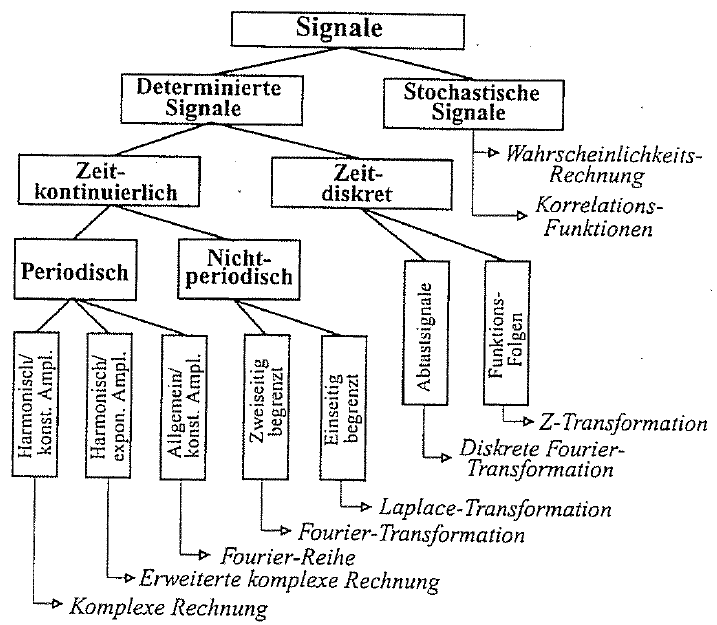
\includegraphics[width=0.8\linewidth]{signale_math_methoden}
	\caption{Signale und mathematische Methoden}
	\label{figure:1}
\end{figure}
\pagebreak

\section{Fourier-Reihen}
\begin{gather*}
	f(t) = c_0 + \sum_{k=1}^{\infty}(a_k\cdot\cos{k\omega t}+b_k\cdot\sin{k\omega t}) \\
	\omega = \frac{2\pi}{T}
\end{gather*}

%\begin{align*}
%	x &= -\frac{p}{2}\pm\sqrt{\left(\frac{p}{2}\right)^2-q}\\
%	f(t) &= c_0 + \sum_{k=1}^{\infty}(a_k\cdot\cos{k\omega t})
%\end{align*}

\begin{table}[h]
	\centering
	%\small\addtolength{\tabcolsep}{+1pt}
	%\setlength\extrarowheight{+5pt}
	%\setlength\tabcolsep{+5}
	\bgroup
	\def\arraystretch{2}
	\begin{tabular}[h]{c|c|c}
		$ \text{auch} -\frac{T}{2} \; \text{bis} \; \frac{T}{2} \; \text{m\"oglich} $ & f\"ur gerade Funktionen & f\"ur ungerade Funktionen \\
		\hline\hline
		$ c_0 = \frac{1}{T}\int_{0}^{T}f(t)\;dt $ & $ c_0 = \frac{2}{T}\int_{0}^{\frac{T}{2}}f(t)\;dt $ & $ c_0 = 0 $ \\
		$ a_k = \frac{2}{T}\int_{0}^{T}\cos(k\omega t)\cdot f(t) \; dt $ & $ a_k = \frac{4}{T}\int_{0}^{\frac{T}{2}}\cos(k\omega t)\cdot f(t) \; dt $ & $ a_k = 0 $ \\
		$ b_k = \frac{2}{T}\int_{0}^{T}\sin{k\omega t}\cdot f(t) \; dt $ & $ b_k = 0 $ & $ b_k = \frac{4}{T}\int_{0}^{\frac{T}{2}}\sin{k\omega t}\cdot f(t) \; dt $ \\
		\hline\hline
		~ & $ f(t) = c_0+\sum_{k=1}^{\infty}a_k\cdot \cos{k\omega t} $ & $ f(t) = \sum_{k=1}^{\infty}b_k\cdot \sin{k\omega t} $
	\end{tabular}
	\egroup
\end{table}

\section{Fourier-Transformation}
\begin{gather*}
	\intertext{FT:}
	F(\omega) = \int_{-\infty}^{\infty}f(t)\cdot e^{-j\omega t}\; dt
	\intertext{IFT:}
	f(t) = \frac{1}{2\pi}\int_{-\infty}^{\infty}F(\omega)\cdot e^{j\omega t}\; d\omega
\end{gather*}

\section{Laplace-Transformation}
\begin{gather*}
	\text{mit} \quad s = \sigma + j\omega
	\intertext{$\mathcal{L}:$}
	F(s) = \mathcal{L}\{f(t)\}(s) = \int_{0}^{\infty}f(t)\cdot e^{-st}\; dt \\
	\intertext{$\mathcal{L}^{-1}:$}
	f(t) = \mathcal{L}^{-1}\{F(s)\}(t) = \frac{1}{2\pi j} \int_{\delta-j\infty}^{\delta+j\infty}F(s)\cdot e^{st}\; ds
\end{gather*}

\pagebreak

\section{Diskrete Fourier-Transformation}
\begin{gather*}
	\intertext{DFT:}
	X[k] = \sum_{n=0}^{N-1}x[n]\cdot e^{-jkn\frac{2\pi}{N}} \\
	\intertext{IDFT:}
	x[n] = \frac{1}{N}\sum_{k=0}^{N-1}X[k]\cdot e^{jkn\frac{2\pi}{N}}
\end{gather*}

\section{Z-Transformation}
\begin{gather*}
	\text{mit} \quad z = e^{T_A \cdot s} = \sigma + j\omega
	\intertext{$Z:$}
	X(z) = Z\{x[k]\} = \sum_{k=0}^{\infty}x[k]\cdot z^{-k}
	\intertext{$Z^{-1}:$}
	x[k] = Z^{-1}\{X(z)\} = \frac{1}{2\pi j}\oint_C X(z)\cdot z^{k-1} \; dz
\end{gather*}

\end{document}